%%%%%%%%%%%%%%%
% EFT Paper
% v.1
% R. Itay & B. Farmer & A. Manfredini
%%%%%%%%%%%%%%%

%\RequirePackage{lineno}
\documentclass[twocolumn, showpacs, showkeys, amsmath, amssymb, amsfonts, floatfix, linenumbers]{revtex4-1} 
\usepackage[colorlinks=true, citecolor=green, filecolor=blue, linkcolor=blue, urlcolor=blue, pdfencoding=auto]{hyperref}
%\usepackage{amsfonts}
\usepackage{color}
\usepackage{placeins} % floatbarrier definition
\usepackage{graphicx}
\usepackage[perpage]{footmisc}
\usepackage[normalem]{ulem}
\newcommand \Leff{\mathcal{L}_{\mathrm{eff}}}
\newcommand \Ly{L_{\mathrm{y}}}
\newcommand \Qy{\mathcal{Q}_{\mathrm{y}}}
\newcommand \keVcc{\mathrm{keV}/\mathrm{c}^2}
\newcommand \keVr{\mathrm{keV_{nr}}}
\newcommand \keVee{\mathrm{keV_{ee}}}
\newcommand{\Xehund}{{XENON100}} 
\newcommand{\Xeten}{{XENON10}}
\newcommand{\Xe}{{\sc Xe}}
\newcommand{\n}[1]{\mathrm{#1}}
\newcommand{\RanComment}[1]{\textcolor{blue}{#1}}
\newcommand{\ale}[1]{\textcolor{red}{#1}}
\newcommand{\BenComment}[1]{\textcolor{green}{#1}}
\newcommand{\Ale}[1]{\textcolor{green}{#1}}
\newcommand{\cc}[1]{$c_{#1}^2\timesm_{Weak}^4$}
\newcommand \Llike{\mathfrak{L}}
\newcommand{\cSi}{\ensuremath{\mathrm{cS1}}}
\newcommand{\cSiib}{\ensuremath{\mathrm{cS2}_\mathrm{b}}}


%%%%%%
% For rendering code example in appendix
\usepackage{listings}
\usepackage{color}
\usepackage{fancyvrb}

\definecolor{dkgreen}{rgb}{0,0.6,0}
\definecolor{gray}{rgb}{0.5,0.5,0.5}
\definecolor{mauve}{rgb}{0.58,0,0.82}

\lstset{frame=tb,
  language=Python,
  aboveskip=3mm,
  belowskip=3mm,
  showstringspaces=false,
  columns=flexible,
  basicstyle={\small\ttfamily},
  numbers=none,
  %numberstyle=\tiny\color{gray},
  keywordstyle=\color{blue},
  commentstyle=\color{dkgreen},
  stringstyle=\color{mauve},
  breaklines=true,
  breakatwhitespace=true,
  tabsize=3
}

%%%%%%%%%

\begin{document}
%\linenumbers 

\title{Effective Field Theory Approach to Scattering of Dark Matter in  \Xehund\ Detector 225 live days run}
%\input{AuthorList}

%\date{\today}

\begin{abstract} 

We report a WIMP search results in \Xehund\ detector considering a non-relativistic effective field theory approach.  The data from scientific run II (34 kg * 224.6 live days) was re-analyzed extending the energy range to 6.6-240~keV. Background and data are found to be compatible. We present 90\% confidence level exclusion limits on the coupling constant of each operator $c_i$ extracted using a binned profile likelihood method. We also consider the case of an inelastic WIMP with more then one mass state scattering and set exclusion limits on this model as well. The presented limits are to date the strongest published limits. 
\end{abstract}

\pacs{}
\keywords{Dark Matter, EFT, Xenon}

\maketitle 


\section{Introduction}
\begin{itemize}
  \item Motivation: dark matter, theoretical possibility of high energy recoil events. Mention some specific models, maybe inelastic scattering also.
  \item Theoretical background on EFT operators, inc. motivation (e.g. possibility to reconcile limits vs possible signals in other experiments, model-independent approach to constraining exotic models)
  \item (if we do it) Theoretical background on inelastic scattering kinematics.
  \item Motivating example plots of recoil spectra/signal models (e.g. Fig. \ref{fig:dRdE}). Also discuss the lower electronic recoil background at these higher recoil energies, which improves the analysis sensitivity beyond what would be expected from the raw increase in predicted event rate (At least I presume so, need to estimate this perhaps. I think we can say something like this; the standard analysis signal region has a signal acceptance of maybe 50\% since it cuts the nuclear recoil band about in half, whereas for us it is almost 90\% since there is good separation between ER and NR bands. So for say O3 (either mass) we expect about twice as many events due to the extended signal region, with twice the acceptance in the new high PE region. So overall I guess it is roughly a factor of 3 improvement in total signal rate, and similar for the sensitivity. In fact from the proper sensitivity estimates the improvement is a little better than that, but this gives a rough idea where the improvement comes from.).

\begin{figure}[h!]
\begin{minipage}{1.\linewidth}
\centerline{\includegraphics[width=1.\linewidth]{Figures/dRdE_examples.pdf}}
\end{minipage}
\caption{Example EFT recoil spectra for elastic scattering of spin-$1/2$ WIMPs on Xenon nuclei (weighted according to the isotope abundances in the XENON100 experiment). Left(right) shows the predicted spectra for EFT operate $O_3$($O_6$). The normalisation is controlled by the coupling coefficient of each EFT operator and the experimental exposure (left arbitrary in this figure). The solid vertical line at 43 keV shows the approximate division between the two signal regions used in this analysis (30 PE in cS1). As shown, certain EFT operators, for certain WIMP masses, predict a significant fraction of recoil events above the upper energy cut used in the standard spin-independent analysis, motivating an extension of this cut. The highest recoil energy shown in the plots, 240 keV, roughly corresponds to the extended $cS1$ cut of 180 PE used in this analysis.}
\label{fig:dRdE}
\end{figure}


\end{itemize}
\section{The \Xehund\  Detector}
The \Xehund\ detector is a cylindrical (30cm height X 30cm diameter) dual phase Xenon Time Projection Chamber (TPC) that holds 62 kg of Liquid \Xe\ (LXe) targets ~\cite{xe100_instr2012}. It operates at the Laboratori Nazionali del Gran Sasso (LNGS) in Italy. The detector consists a total of 242 1”-square Hamamatsu R8520-AL photomultiplier tubes (PMTs) employed in two arrays, at the top part (in the gas phase) and in the bottom immersed in LXe. a Particle interacting with the LXe deposits energy that creates both excited and ionized states. De-excitation creates a prompt scintillation signal ($S1$). ,  Ionized electrons are drifted in an electric field of $530$V/cm towards the liquid-gas interface, where they are extracted via a larger electric field of $\sim12$kV/cm. These electrons generates a proportional scintillation, which is called $S2$. The spatial distribution of the $S2$ signal on the top PMT array, determines the X-Y position, while the time difference between the two signals gives the z-coordinate, and thus a 3D position reconstructions is achieved.

The ratio of S2/S1 is different weather the interaction is nuclear recoil (NR) or electronic recoil (ER) and thus this ratio is used as a discriminator between ER background coming from $\gamma$, $\beta$ and NR signal coming from a WIMP. 

In previous \Xehund\ analyses the determination of the recoil energy was based on the size of S1 and the scintillation efficiency for the nuclear recoils, \Leff ~\cite{xe100_run10_si}. However in the last analysis ~\cite{xe100_run_combination} a new method was adopted taking into advantage also the S2 signal.
      



\section{Data Analysis}
\label{sec:Analysis}
In this work we re-analyze scientific run~II data recorded between February 2011 and March 2012, 
corresponding to 224.6~live~days. The characterization of the detector response to ER interactions is performed using dedicated calibration campaigns with $^{60}$Co and $^{232}$Th radioactive sources, while the response to NR interactions is performed using $^{241}$AmBe calibration campaigns.
%\sout{as well as for estimating the background from $\beta$ and $\gamma$-particles. For the ER sample we expose the detector to $^{60}$Co and $^{232}$Th sources, while for the NR sample we use $^{241}$AmBe.}

 
This work extends the previous results~\cite{xe100_run10_si,xe100_run_combination}, referred to in the following as the low energy channel, with a new study exploring the recoil energy range between 43-240\,keV. 
The data analysis is divided into two mutually exclusive channels, one optimized for low energies and ranging from 3-30\,PE in cS1 (lowE), 
the other optimized for high energies recoils ranging from 30-180\,PE in cS1 (highE).  These two analysis are then statistically combined. 
The regions of interests (ROI) in these two channels, in which we search for dark matter events, are shown in Figure~\ref{fig:phasespace} and further described in the following sections. 


\subsection{Low Energy}
\label{subsec:LowE}
This analysis take advantage of the previous result~\cite{}, the analysis format, meaning the background model, data selections and their acceptances, 
statistical interpretation of data, is kept unchanged and only briefly summarized here. The only exception is the signal model production where 
minor differences are highlighted in Section~\ref{subsec:SignalModel}.

The region of interest for this channel.....
Those bands are defined based on a simulated signal model, arranged in order to have equal signal density in each.

Other than falling into the ROI an event should fullfill several other selection criteria such as, data quality cuts,
veto for events with energy release in the outer LXe shield, selection of single-scatter event, energy selection, S2 threshold cut and 
a predefined fiducial volume of 34\,kg. Details on these selections and on their relative acceptances on WIMP signals are detailed in~\cite{Aprile:2012vw}. 
Sentence on the advanced cuts.

Background model....




\subsection{High Energy}
\label{subsubsec:HighE}
This analysis channel targets high energy nuclear recoils and is the focus of this work. The data selection criteria we use are based on the criteria described in detail in \cite{Aprile:2012vw}, which were optimized for high 
acceptance to low energy nuclear recoils.
Most of these selection criteria (cuts) were found to be fully compatible with (or easily extended) to high energy depositions, however some required more comprehensive studies, which are described in what follows. 

%very nice!
The width of an S2 pulse increases with the depth (z) of the interaction. This is due to the diffusion of the electron cloud during its propagation
towards the gate grid. Low energy S2 events show larger spread
due to low statistics of drifted ionization electrons, hence
the cut was previously defined in an energy-dependent way. However for recoil energies which are high enough, as in this channel, this energy dependency is not valid. We therefore use here a cut on the S2 width which is a function of the depth of the interaction alone. 
%\textbf{I can add a comment stating that the main differance is that we set S2sTot[0] =  5000 for any value above 5000, but I think it is not needed.}}
%To reject peculiar events we compare the width of the S2 to its z-position. In this analysis we adopt a newer version of this cut, developed for scientific run III, see ~\cite{xe100_run_combination}, \Ale{can't you just paste what's written there for this cut} \RanComment{suprisingly no it is not described there , so either we do not describe it as well or keep it like this.}. 

As a WIMP will interact only once in the detector, we remove events which have more than one S2. We adopt here a cut that is more suitable to higher energies and demands a single S2 in a 160 $\mu$S window, instead of a linear dependence between the second S2 size and the first. 

To define the interaction's exact location, we use several algorithms, one of which is based on a Neural Network (NN)~\cite{Aprile:2012vw}. The NN was not trained to recognize high energy ER events and therefore a cut on the NN score is not suitable for this analysis. We therefore discard this cut but keep all other cuts on position reconstruction quality, which is sufficient to ensure a correct position reconstruction. 

The total acceptance to WIMP signals is computed based on $^{241}$AmBe calibration data as a function of cS1, following the procedure described in~\cite{Aprile:2012vw}. We present this function in Figure~\ref{fig:Acc}, where the total acceptance is fitted using a 3rd order polynomial.

\begin{figure}[t!]
\begin{minipage}{0.9\linewidth}
\centerline{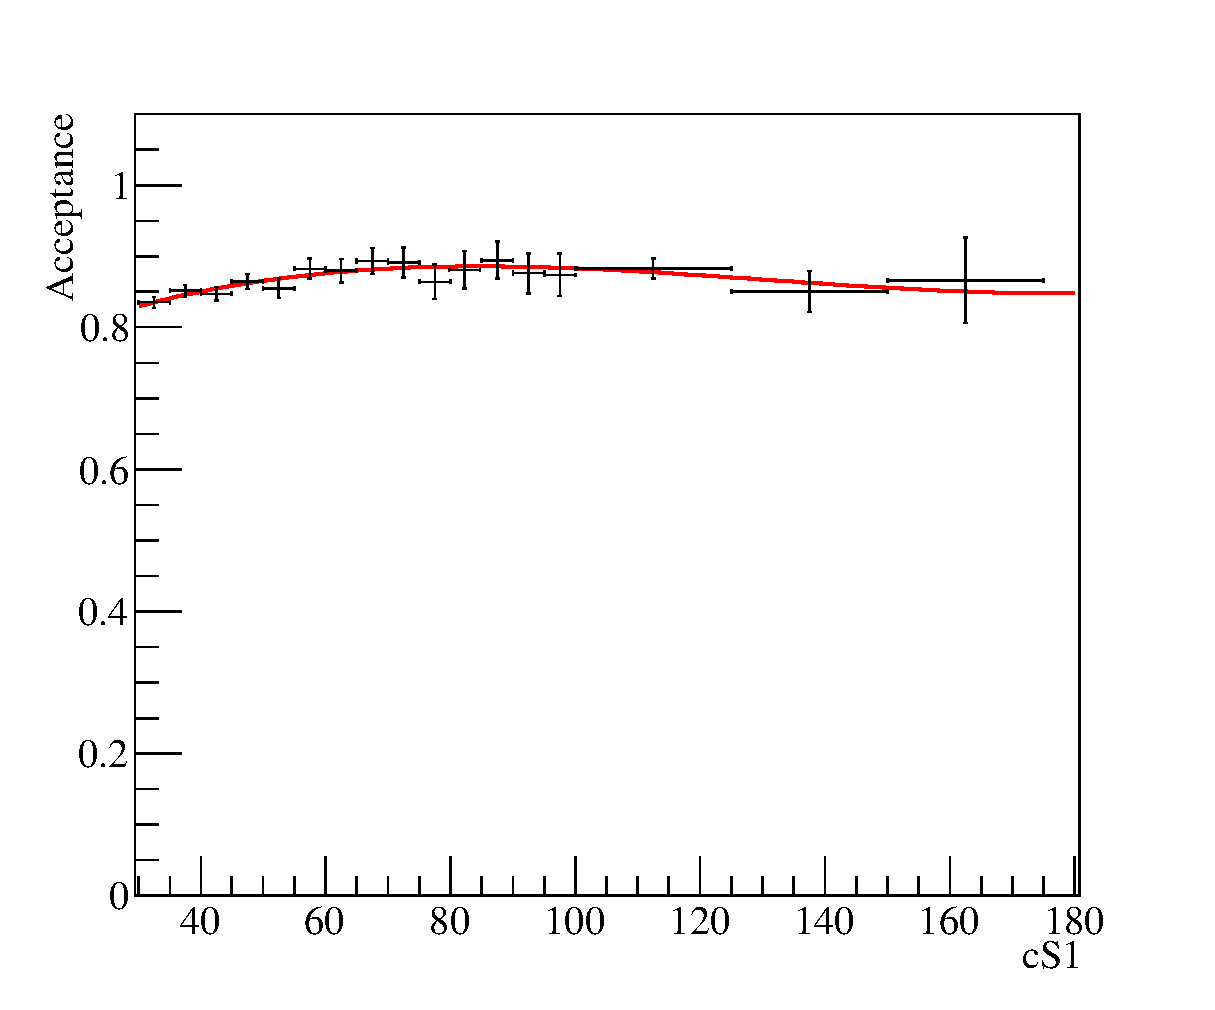
\includegraphics[width=1.\linewidth]{Figures/Acceptance.eps}}
\end{minipage}
\caption{The total acceptance of all cuts used. Data from calibration is shown in black, with a polynomial fit in red.}
\label{fig:Acc}
\end{figure}

We define our signal region in the discrimination (y,cS1)-plane using $^{241}$AmBe calibration data. 
The ROI is shown in Figure~\ref{fig:phasespace} as blue contour lines: the upper bound is defined such that it is not contaminated from contribution due to xenon excitation lines, the lower is defined as the 3\,$\sigma$ acceptance quantile of the $^{241}$AmBe distribution.

We divide our signal region into two bands, constructed such that the $^{241}$AmBe data sample is equally distributed in y between them. The total number of events in each band is $\sim3000$ events. The bands are further divided into nine bins. The definition and content of the bins are presented in Table~\ref{table:BinDef} and in Figure~\ref{fig:phasespace}. 


%%%%%%%%%%%%%%%%%%%%%%%%%%%%%%%%%%%%%%%%%%%%%%%%%%%%%%%%%%%%%%%%%%%%%%%%%%%%%%%%%%%%%%%%%%%%%%%%%%%%%%%

%%%%%%%% THIS PROBABLY NEEDS A SECTION, explaining well the uncertainty determination %%%%%%%%%%%%%%%%%
The main source of background results from ER leakage, therefore we estimate the background distribution in the ROI using $^{60}$Co and $^{232}$Th calibration samples.  
Contributions from radiogenic and cosmogenic neutrons, and accidental coincidence, are negligible for such a high energy recoil. In Table~\ref{table:BinDef} we report the background expectation for each bin in the ROI along with the observed events in each bin. The background expectation is computed by scaling the calibration sample yield by $6.54\times10^{-3}$, which is simply the ratio of observed counts to calibration counts in an independent sideband. Note that the background normalization is fitted to data during hypothesis testing, as described in section~\ref{sec:LikelihoodFunction}. 

%%%%%%%%%%%%%%%%%%%%%%%%%%%%%%%%%%%%%%%%%%%%%%%%%%%%%%%%%%%%%%%%%%%%%%%%%%%%%%%%%%%%%%%%%%%%%%%%%%%%%%%


\begin{table}
\resizebox{1.\columnwidth}{!}{

	 \begin{tabular}{|c| c| c| c| c| c |} 
 \hline
 \# & Band  & Energy Range (cS1)  & \# Background Events & \# Data Events \\  
 \hline\hline
 1 & upper & 30  - 40  & 23.5 & 20 \\ 
 \hline
 2 & upper & 40  - 50  & 15.7 & 17 \\
 \hline
 3 & upper & 50  - 80  & 12.4 & 11 \\
 \hline
 4 & upper & 80  - 120 & 1.1  & 1  \\
 \hline
 5 & upper & 120 - 150 & 0.1  & 1  \\  
 \hline
 6 & upper & 150 - 180 & 0.08 & 0  \\  
 \hline
 7 & lower & 30  - 50  & 0.9  & 0  \\  
 \hline
 8 & lower & 50  - 90 & 0.35 & 0  \\  
 \hline
 9 & lower & 120 - 180 & 0.18 & 0  \\  
 \hline
\end{tabular}
}

\caption{Definitions and contents of the analysis bins for the high energy channel. The expected background counts are calculated by taking the calibration sample and scaling it by $6.54\times10^{-3}$, which is the ratio of observed counts to calibration counts in a sideband.}  \label{table:BinDef} 
\end{table}


\begin{figure}[]
\begin{minipage}{1\linewidth}
\centerline{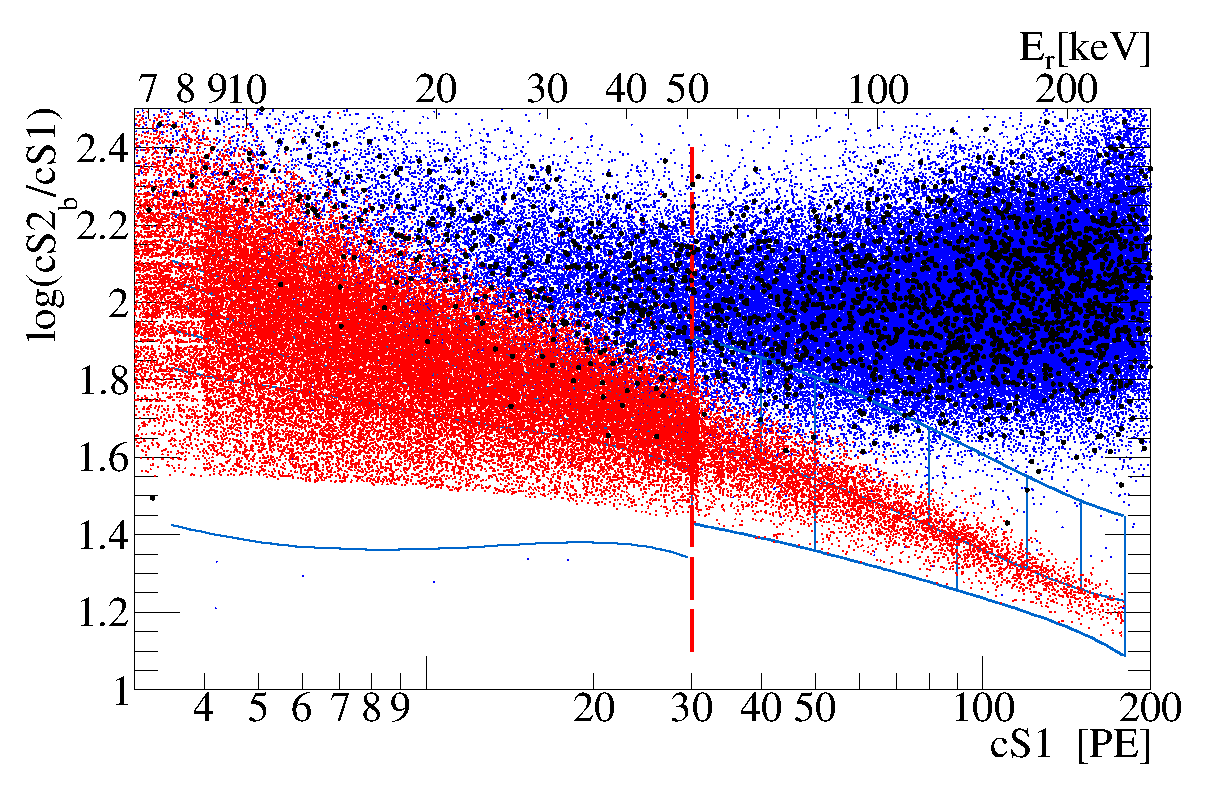
\includegraphics[width=1\linewidth]{Figures/eft_sr.eps}}
\end{minipage}
\caption{Summary of regions of interest, backgrounds, and observed data. ER calibration data, namely $^{60}\mathrm{Co}$ and $^{232}\mathrm{Th}$ data is shown as blue dots. NR calibration data ($^{241}$AmBe) is shown as red dots. Dark matter data is shown as black dots. The red dashed line is the threshold between the low and high energy channels. The lines in blue are the bands. For the low energy channel the shown bands are constructed for a 50 GeV/$c^2$ WIMP. For the high energy region the 9 analysis bins are presented; the top left bin in this region is bin 1, the top right is bin 6, the bottom left is bin 7 and bottom right is bin 9. In Appendix~\ref{app:1000PE} we show similar data but for regions above the upper range of this analysis, going up to 1000\,PE in cS1, for the sake of curiosity as part of final unblinding of XENON100 data. 
}
\label{fig:phasespace}
\end{figure}  




\subsection{Signal Model}
\label{subsec:SignalModel}
The signal model is produced by taking a theoretical event rate spectrum, the production of which is described in sections \ref{subsubsec:Elastic} and \ref{subsubsec:Inelastic}, and applying the analysis acceptance and detector response as described in ~\cite{Aprile:2012vw}  to obtain the expected event rate in the detector in terms of detector variables (i.e. cS1,cS2). In order to calculate the expected value of the signal in cS1, we use Eq.~\ref{eq:LeffEnergyScale} for both energy regions, 
\begin{equation}
\label{eq:LeffEnergyScale}
	\langle cS1 \rangle = E_{\mathrm{nr}} \cdot (\Ly \Leff) \cdot   \left(\frac{S_{nr}}{S_{ee}}\right) 
\end{equation}
%\begin{multline}
%\label{eq:low2D}
%  \frac{\mathrm{d}^2 R}{\mathrm{d}\cSi.\mathrm{d}\cSiib} = \epsilon_\mathrm{S1}(\cSi).\epsilon_\mathrm{S2}(\cSiib) \\ 
%  \times \int \! \frac{\mathrm{d}R}{\mathrm{d}E}.p_\mathrm{S1}(\mathrm{\cSi}|E).p_\mathrm{S2}(\mathrm{\cSiib}|E) \, \mathrm{d}E
%\end{multline}

%where
%
%\begin{align}
%\label{eq:S1S2pdf}
% p_\mathrm{S1}(\mathrm{\cSi}|E) &= \sum_{N'} P_\mathrm{pmt}(\mathrm{\cSi}|N',0.5 \sqrt{N'}).\mathrm{Pois}(N'|\mu_\gamma) \\
% p_\mathrm{S2}(\mathrm{\cSiib}|E) &= \sum_{N'} P_\mathrm{pmt}(\mathrm{\cSiib}|Y N',\sigma_Y \sqrt{N'}).\mathrm{Pois}(N'|\mu_Q)
%\end{align}
%
%where $P_\mathrm{pmt}$ is a normal distribution with arguments as $N(x|\mu,\sigma)$, and where
%
%\begin{align}
%\mu_\gamma(E) &\approx E \cdot L_y \cdot L_\mathrm{eff}(E) \cdot \frac{S_\mathrm{nr}}{S_\mathrm{ee}} \\
%\mu_Q(E) &\approx Q_y(E) \cdot E
%\end{align}

where $E_\mathrm{nr}$ is the recoil energy, $\Ly$ is the detector related light yield, $\Leff$ is the scintillation efficiency relative to 122$\keVee$ as a function of $E_\mathrm{nr}$, and $S_{ee}$ and $S_{nr}$ are the quenching factors for ER and NR respectively. Aside from $E_\mathrm{nr}$ and $\Leff$ these parameters have fixed values, namely $\Ly = 2.28 \pm 0.04$, $S_\mathrm{nr} = 0.95$, and $S_\mathrm{ee} = 0.58$. Recoils below 3 keV are assumed to produce no light since $\Leff$ is not measured at these energies. For details of the physics behind these parameters and the construction of the signal PDF please see \cite{Aprile:2012vw,xe100_run_combination}. 

The expected cS2 signal is computed following~\cite{DataMCXenon} using Eq.~\ref{eq:Qy} for the lowE region only,
%For the lowE region, the expected cS2 signal can be calculated as well~\cite{DataMCXenon} using Eq.~\ref{eq:Qy},
%
\begin{equation}
\label{eq:Qy}
	\langle cS2_{bottom} \rangle = E_{\mathrm{nr}}\Qy Y   
\end{equation}
%
%where $Y = 8.4366$   %where did you thake this number??
where $Y = 8.27 \pm 0.26$ 
is the amplification factor determined from the detector response to single electrons~\cite{XenonSingleElectron}, and $\Qy$ is the charge yield as a function of $E_\mathrm{nr}$. Note that as some of the top PMTs saturate we use only the bottom PMT for energy scale in S2. Applying the detector and PMT responses, and the acceptance as in \cite{xe100_run_combination}, defines the lowE signal model over the region $3 \mathrm{PE} < \cSi < 30 \mathrm{PE}$, with $\cSiib > 73.5 \mathrm{PE}$.

%%%%%%%%%%%%%%%%%%%%%%%%%%%%%%%%%%%%%% THIS PART IS NOT NEEDED  Ale votes for removal %%%%%%%%%%%%%%%%%%%%%%%%%%%%%%%%%%%%%%%%%%%%%%%%%%%%
Eq. \ref{eq:Qy} hides a small subtlety. The actual $cS2_{bottom}$ PDF is composed of two pieces, a Poisson term associated with the initial charge liberation and a Gaussian term associated with the PMT response and other detector effects:
%
\begin{equation}
\label{eq.cS2pdf}
p_\mathrm{S2}(\mathrm{\cSiib}|E) = \sum_{N'} P_\mathrm{pmt}(\mathrm{\cSiib}|Y N',\sigma_Y \sqrt{N'}).\mathrm{Pois}(N'|\mu_Q)
\end{equation}
%
where $\mu_Q=E_{\mathrm{nr}}\Qy$ is the expected number of liberated charges in a nuclear recoil event of energy $E$, and $N'$ is the actual number of liberated charges, which are unmeasured and thus summed over. The amplification factor $Y$ is applied on the actual number of liberated charges $N'$, not the expected number $\mu_Q$. Associated with this is the variance of the Gaussian response PDF, $\sigma_Y\sqrt{N'}$, where in this analysis $\sigma_Y = 6.93$. 
%%%%%%%%%%%%%%%%%%%%%%%%%%%%%%%%%%%%%%%%%%%%%%%%%%%%%%%%%%%%%%%%%%%%%%%%%%%%%%%%%%%%%%%%%%%%%%%%%%%%%%%%%%%%%%%%%%

For the high energy region we can not produce the S2 distribution as the method in~\cite{DataMCXenon} is not calibrated for high enough recoil energies. We therefore use the NR calibration data distribution in log($\mathrm{cS2_b/cS1}$) to estimate the WIMP one. Above 180PE in \cSi\ the statistics of $^{241}$AmBe data is too low to estimate the distribution accurately so this forms the higher bound of this analysis. With the \cSiib\ distribution determined by this empirical method we require only a prediction of the \cSi\ distribution. This is obtain from Eq. \ref{eq:LeffEnergyScale}, followed by the application of detector and PMT responses, as well as the acceptance given in~\ref{fig:Acc}, which completes the highE signal model definition.

Examples of each for two EFT operators are shown in Figures ~\ref{fig:HighE} and \ref{fig:LowE}, with the rate normalized to give 5 events in the total energy range (lowE and highE).

\begin{figure}[h!]
\begin{minipage}{1.\linewidth}
\centerline{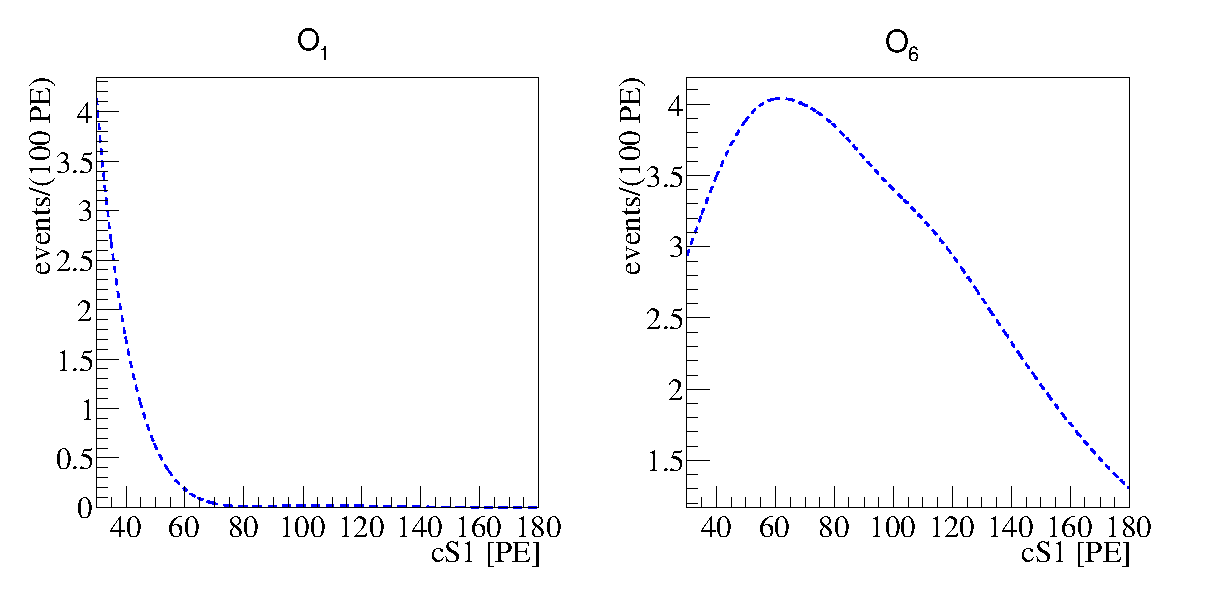
\includegraphics[width=1.\linewidth]{Figures/SigHighO1O6.eps}}
\end{minipage}
\caption{The expected signal in the high energy region for a 300 GeV/$c^2$ WIMP mass, Normalized to 5 events. Left(right) is the spectra for $O_1$($O_6$). Notice that for $O_1$ most of the events are not expected to deposit energy higher then 30 PE whereas for $O_6$ a large fraction of the events appear in this region.}
\label{fig:HighE}
\end{figure} 

\begin{figure}[h!]
\begin{minipage}{1.\linewidth}
\centerline{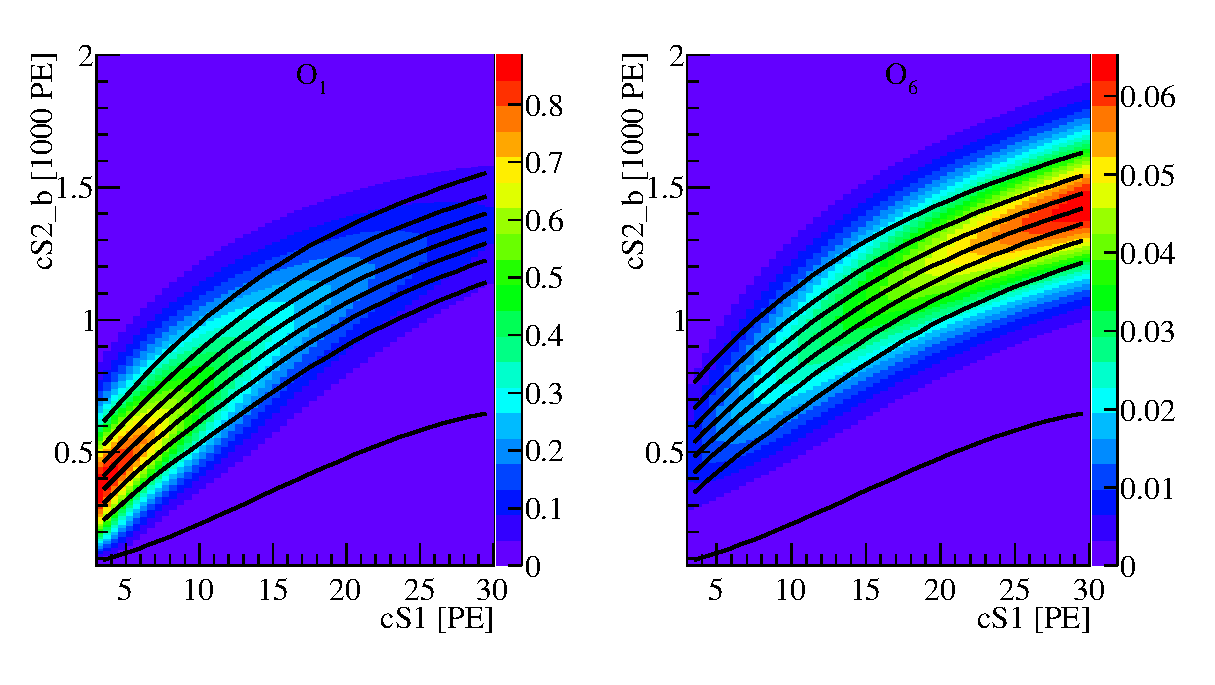
\includegraphics[width=1.\linewidth]{Figures/SigLowO1O6.eps}}
\end{minipage}
\caption{The expected signal in the low energy region for a 300 GeV/$c^2$ WIMP mass, Normalized to 5 events. Left(right) is the spectra for $\mathcal{O}_1$($\mathcal{O}_6$). Notice that for $\mathcal{O}_1$ most of the events are expected to deposit energy lower then 30 PE whereas for $\mathcal{O}_6$ a large fraction of the events do not appear in this region at all. The black lines indicate the bands constructed on this specific event rate, and are dividing the signal into 8 equally distributed signal sub-regions.}
\label{fig:LowE}
\end{figure}




%
%\begin{multline}
%\label{eq:high2D}
%  \frac{\mathrm{d} R}{\mathrm{d}\cSi} = \epsilon_\mathrm{S1}(\cSi) \int \! \frac{\mathrm{d}R}{\mathrm{d}E}.\epsilon_\mathrm{S2'}(E).p_\mathrm{S1}(\mathrm{\cSi}|E) \, \mathrm{d}E
%\end{multline}

%\sout{
%where $p_\mathrm{S1}(\mathrm{\cSi}|E)$ is computed as in Eq. \ref{eq:S1S2pdf}. The S1 acceptance $\epsilon_\mathrm{S1}(\cSi)$ is given in Fig. \ref{fig:Acc}, and the S2 acceptance $\epsilon_\mathrm{S2'}(E)$ is negligibly different from one over the signal region $30 \mathrm{PE} < \cSi < 180 \mathrm{PE}$.
%}
\subsubsection{Elastic Scattering}
\label{subsubsec:Elastic}

The expected recoil energy spectrum of each WIMP mass for each EFT operator is calculated using the Mathematica package \texttt{DMFormFactor} supplied by Anand et. al.~\cite{Fitzpatrick:MathTools,Anand:MathTools}. We use standard assumptions as in previous analyses (e.g \cite{xe100_run_combination}) regarding the local dark matter density and velocity distribution, namely $\rho_\mathrm{local} = 0.3$ GeV/cm\textsuperscript{3} and a Maxwell-Boltzman distribution with a mean given by the local circular velocity $v_0 = 220$ km/s and cut off at an escape velocity of $v_\mathrm{esc} = 544$ km/s. The responses of Xe nuclei to a scattering event are computed from one-body density matrices provided with the package, in contrast to the Helm form factors which have been used in previous analyses. These spectra are produced for the seven most abundant Xe isotopes (128,129,130,131,132,134 and 136), combined in proportion to the abundance of these isotopes in the experiment \cite{xe100_run10_sd}, then translated into expected signal rates via the method described above.

\subsubsection{Inelastic WIMP Scattering}
\label{subsubsec:Inelastic}
To obtain recoil spectra for WIMP-nucleon scattering for all EFT operators with inelastic kinematics, we use a modified version of \texttt{DMFormFactor} provided by Barello et. al. \cite{InelasticMath}. The authors have modified the original package to enforce the new energy conservation condition $\delta_m + \vec{v}\cdot\vec{q} + \left|\vec{q}\right|^2/2\mu_N = 0$, primarily by replacing 
$\vec{v}^\perp_{elastic} \rightarrow \vec{v}^\perp_{inelastic} = \vec{v}^\perp_{elastic} +\frac{\delta_m}{\vert{\vec{q}}\vert^2}\vec{q}$ in the definitions of the EFT and nuclear operators, giving rise to the well-known minimum velocity for scattering
\begin{equation}
  v_\mathrm{min} = \frac{1}{\sqrt{2 m_N E_R}} \left|\frac{m_N E_R}{\mu_N} + \delta_m\right|
\end{equation}
where $\mu_N$ is the WIMP-nucleon reduced mass.

Assumptions regarding the dark matter halo and nuclear physics are unchanged. The mass splitting $\delta_m$ between dark matter states is varied from 0 to 300 keV, safely beyond the value at which the predicted rate is zero for the entire mass range we consider.


\subsection{The Likelihood Function}
Explanation of the likelihood methods used, short explaination of the likelihood parts and constraints for combination, joint usage of nuisance parameters {Leff}.
%\subsubsection{High Energy}
%likelihood function + uncertainties 
%\subsubsection{Low Energy}
%ref to run combination.



\section{Results}
\label{sec:Results}
%\subsection{Elastic Scattering}

A benchmark region of interest is defined between the upper and lower thresholds in \cSi{} for each channel. This region
is bounded in $y$-space from above by the $^{241}$AmBe NR mean line and below by the lower 3$\sigma$ quantile of the $^{241}$AmBe neutron calibration data. The expected background in the region is $3.0 \pm 0.5_{stat}$ (low-energy) and $1.4 \pm 0.3_{stat}$ (high-energy). The number of DM candidates in this benchmark region is 3 (low-energy), and 0 (high-energy). Consequently, the data is compatible with the background-only hypothesis and no excess is found. 

For the elastic scattering case, a 90\%\,CL$_S$~\cite{cls} confidence level limit is set on the effective coupling constant, $c_i$,  for all operators and masses in the range of 10~GeV/$c^2$ to 1 TeV/$c^2$. The $c_i$ are dimensionful, with units of $[\mathrm{mass}]^{-2}$, so we first convert them to dimensionless quantities by multiplying them by $m_\mathrm{weak}^2=(246.2\text{ GeV})^2$, following the conventions of \cite{Anand:MathTools}. 

These limits are shown in Fig.~\ref{fig:elasticLimit} in black, along with limits from CDMS-II Si, CDMS-II Ge and SuperCDMS~\cite{CDMSEFT}.  


For the inelastic scattering case,  90\%\,CL$_S$ confidence level limits on the coupling constants 
(again scaled by $m_\mathrm{weak}^2$) are set. Fig.~\ref{fig:O1Inel} shows limits on the $\mathcal{O}_1$ (SI) coupling constant as a function of mass splitting and WIMP mass, Fig.~\ref{fig:InelasticLimit} shows limits for all other operators as a function of the mass splitting $\delta_m$ with a fixed WIMP mass of 1 TeV/$c^2$,  
projections of results from CDMS-II~\cite{CDMS_Inelastic}, ZEPLIN-III~\cite{Zepplin_Inel}, and \Xehund~\cite{XENON_Inelastic_WIMP} in the coupling constant and $\delta_m$ parameter space are also reported.
  

\begin{figure*}
\begin{minipage}{1.\linewidth}{}
\centerline{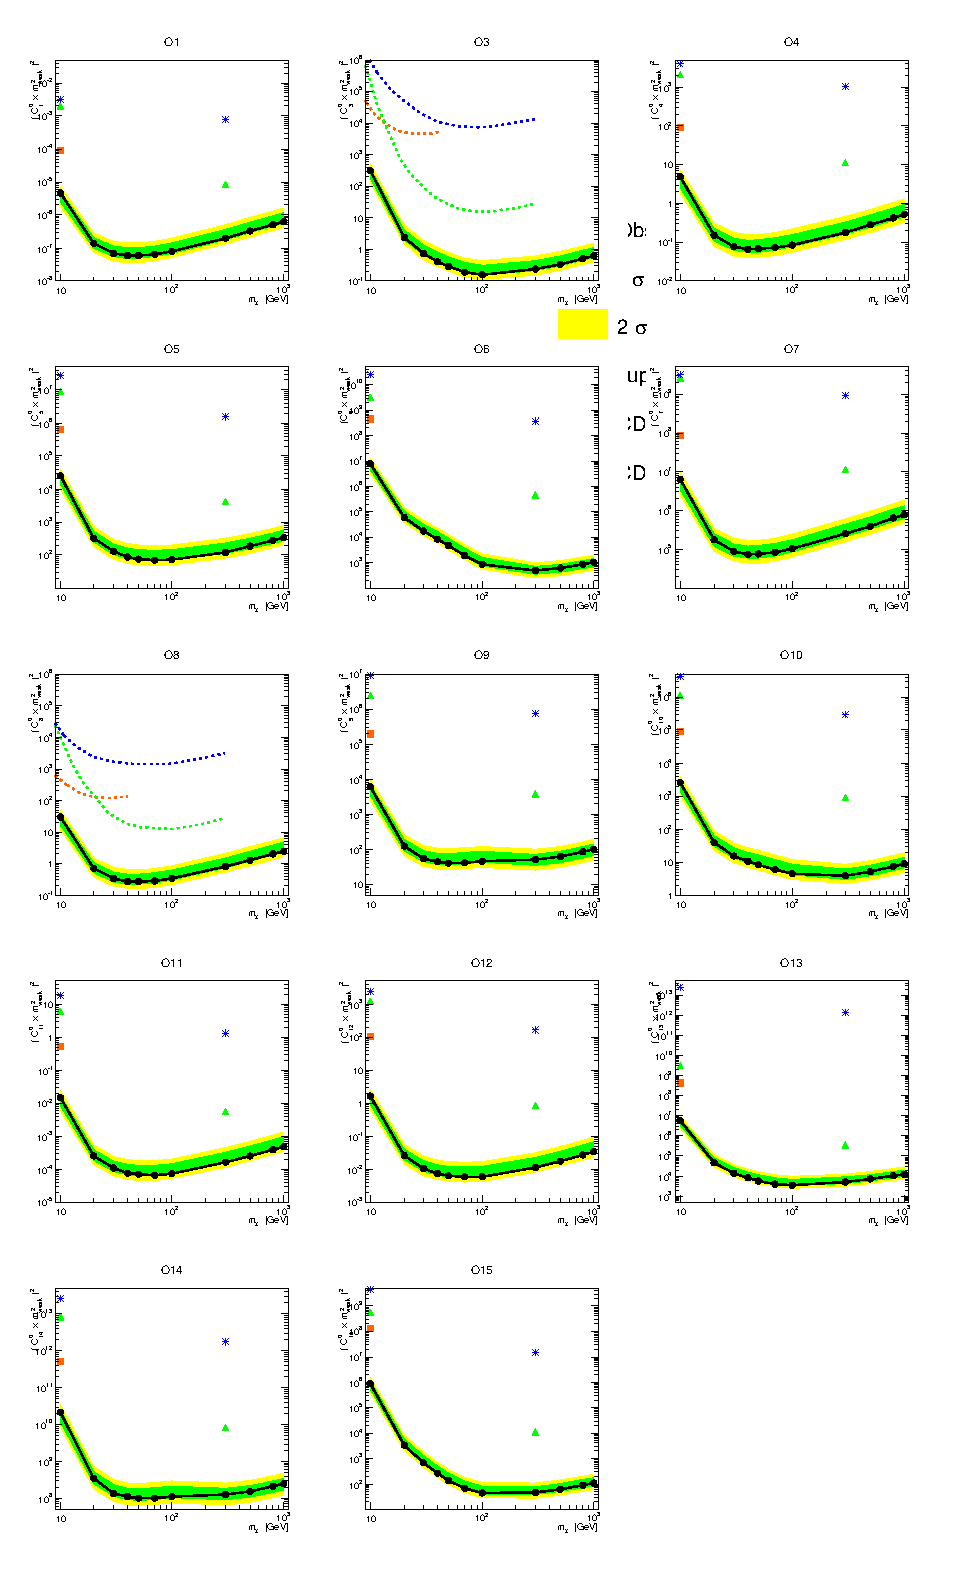
\includegraphics[width=\textwidth,height=0.99\textheight,keepaspectratio]{Figures/ElasticAllLimitCDMS.eps}}
\end{minipage}
\caption{The \Xehund\ limits (90\%\,CL$_S$) on isoscalar dimensionless coupling for all elastic scattering EFT operators. The limits are indicated in solid black. The expected sensitivity is shown in green and yellow(1$\sigma$ and 2$\sigma$ respectively). Limits from CDMS-II Si, CDMS-II Ge, and SuperCDMS \cite{CDMSEFT} are presented as blue asterisks, green triangles, and orange rectangles, respectively (color online). For operator 3 and 8 a full limit was published, for all other operators only $m_\chi = 10$ and $m_\chi =300$ are available.}
\label{fig:elasticLimit}
\end{figure*}

\begin{figure}
\centerline{\includegraphics[width=1.\linewidth]{Figures/O1_inelastic_lim_2D}}
\caption{90\%\,CL$_S$ limits, for the inelastic model, on the magnitude of the coupling constant for $\mathcal{O}_1$, reported as a function of the WIMP mass and mass splitting $\delta$.}
\label{fig:O1Inel}
\end{figure}  


\begin{figure*}
\begin{minipage}{1.\linewidth}
\centerline{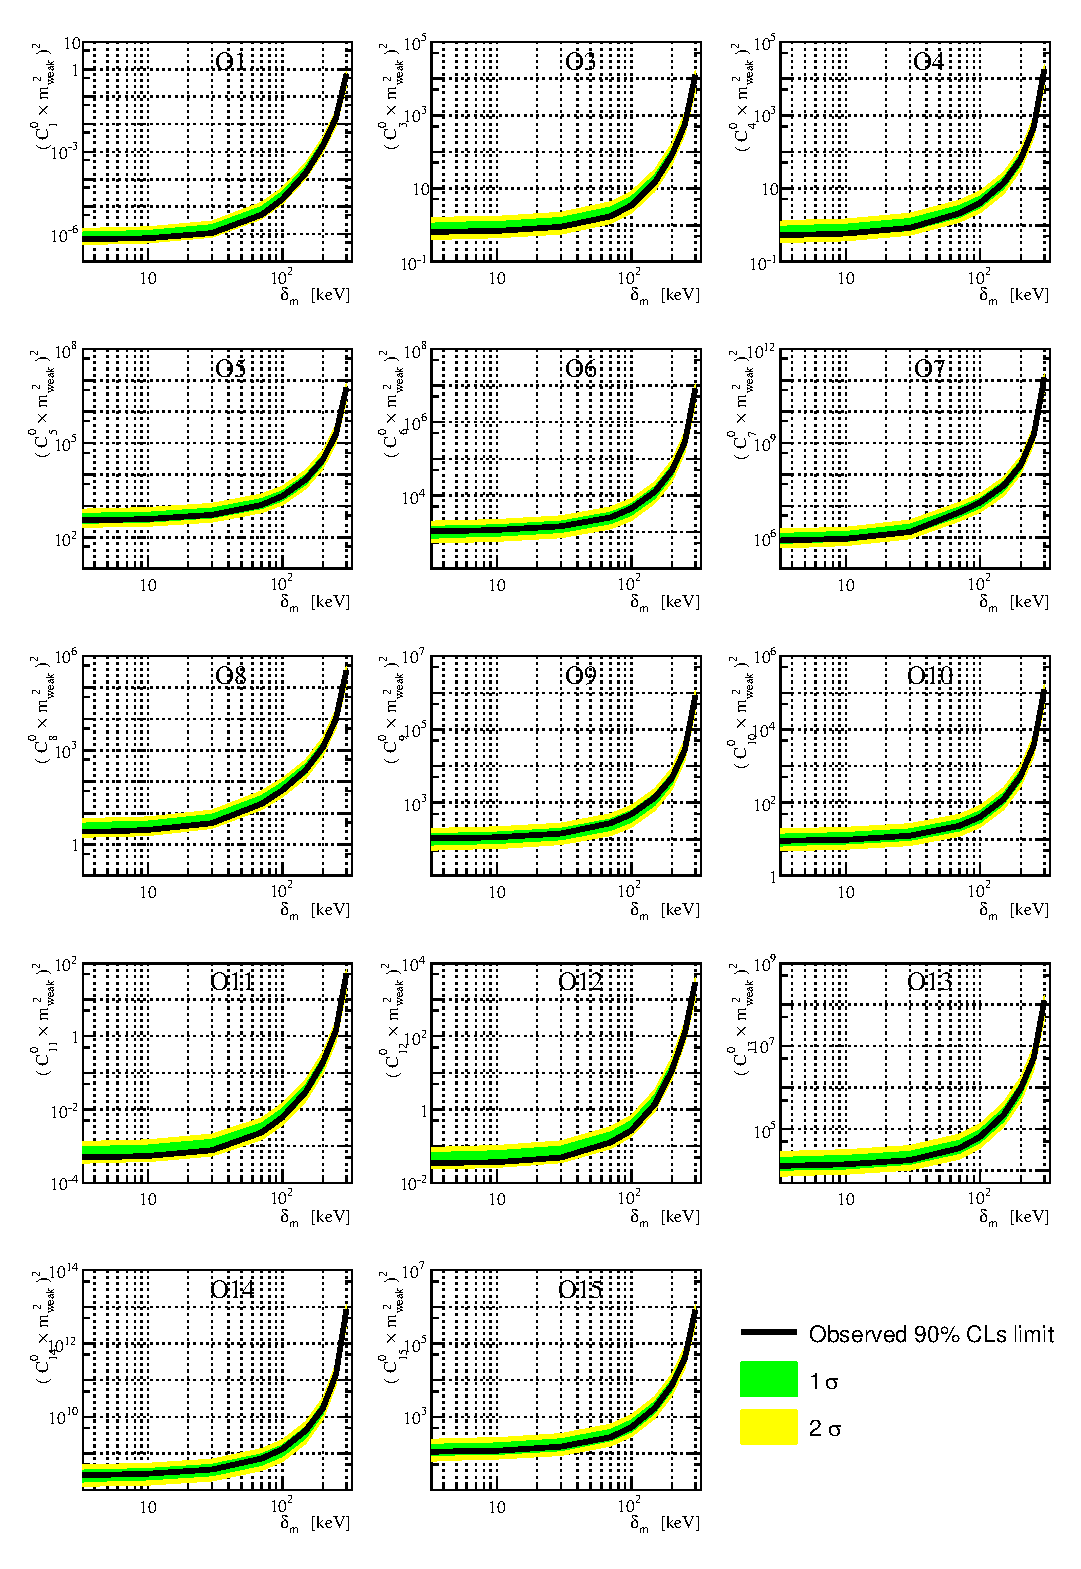
\includegraphics[width=\textwidth,height=0.99\textheight,keepaspectratio]{Figures/FinalInelastic.eps}}
\end{minipage}
\caption{The \Xehund\ 90\%\,CL$_S$ limits on a 1 TeV/$c^2$ WIMP isoscalar dimensionless coupling constant as function of the WIMP mass splitting $\delta_m$  for all inelastic scattering EFT operators. Limits are indicated in solid black. The expected sensitivity is shown in green and yellow (1$\sigma$ and 2$\sigma$ respectively). For $\mathcal{O}_1$ (SI) results from \Xehund(red triangle) CDMS-II(blue rectangle) and ZEPLIN-III(black star) are overlaid.}
\label{fig:InelasticLimit}
\end{figure*}

For the elastic operator $O_1$ our results can be compared to those of standard SI analyses by computing the relevant zero-momentum WIMP-nucleon cross-sections. This is not simple to do rigorously because the treatment of nuclear structure used in our analysis is different than in standard analyses, however this difference is small for scattering via $O_1$. We can therefore quite safely use the `traditional' correspondence~\cite{DeSimone:2016fbz}
%
\begin{equation}
\sigma_{N}^\mathrm{SI} = \left(C^N_1\right)^2 \frac{\mu_{\chi,N}^2}{\pi}
\end{equation}
%
where $\mu_{\chi,N}$ is the WIMP-nucleon reduced mass. Standard SI analyses assume isospin-conserving interactions, as we do in this analysis, so we can simply set $C^N_1 = C^0_1$, such that $\sigma_{p}^\mathrm{SI}=\sigma_{n}^\mathrm{SI}$. 

In principle a similar comparison can be done between our limit on the $O_4$ coupling and standard SD analysis limits, however this time the standard analyses do {\em not} assume isospin-conserving interactions. Instead they typically assume maximal isospin violation, that is, assuming that WIMPs couple either protons or neutrons. Limits are then derived independently on $\sigma_{p}^\mathrm{SD}$ and $\sigma_{n}^\mathrm{SD}$. Because of this difference in assumptions, our limits on SD couplings are not directly comparable to usual analyses. However, they can be recast under the appropriate alternate model assumptions using the detector response tables we provide in the supplementary material.
 

\section{Summary}
We have shown the first analysis of \Xehund\ data at recoil energies above 43 keV, with the new high energy bound set to 240 keV. We considered in this paper two models which predict interactions in this energy region: an EFT approach for elastic WIMP-nucleon scattering, and a similar EFT approach but considering instead inelastic WIMP-nucleon scattering. The observed data was compatible with background expectations, and 90\%\,CL$_S$ exclusion limits were constructed for WIMP masses between 10-1000 GeV.

\begin{acknowledgments}
We would like to thank Andrew Liam Fitzpatrick and Spencer Chang for supplying and helping with their Mathematica packages . We gratefully acknowledge support from the National Science Foundation, Swiss National Science Foundation, Deutsche Forschungsgemeinschaft, Max Planck Gesellschaft, German Ministry for Education and Research, Netherlands Organisation for Scientific Research, Weizmann Institute of Science, I-CORE, Initial Training Network Invisibles (Marie Curie Actions, PITNGA-2011-289442), Fundacao para a Ciencia e a Tecnologia, Region des Pays de la Loire, Knut and Alice Wallenberg Foundation, Kavli Foundation, and Istituto Nazionale di Fisica Nucleare. We are grateful to Laboratori Nazionali del Gran Sasso for hosting and supporting the XENON project.
\end{acknowledgments}

%\newpage



\appendix
\section{Signal model detector response table}

In this appendix we describe digital tables which can be used to construct an accurate signal model for this analysis given any input recoil spectrum $\mathrm{d}R/\mathrm{d}E$. A visualisation of the tables is shown in Fig. \ref{fig:smeartable_highE}, and in section \ref{app:example_code} we show a simple example of how to use the supplied tables in Python. Currently we provide these tables only for the high E analysis region.

The signal model for the high E analysis region can be expressed analytically in the form:
%
\begin{align}
\label{eq:high2D}
  \frac{\mathrm{d} R}{\mathrm{d}\cSi} &= \int \! \frac{\mathrm{d}R}{\mathrm{d}E}.\epsilon_\mathrm{S1}(\cSi) .\epsilon_\mathrm{S2'}(E).p_\mathrm{S1}(\mathrm{\cSi}|E) \, \mathrm{d}E \\
  &= \int \! \frac{\mathrm{d}R}{\mathrm{d}E} G(\cSi,E) \, \mathrm{d}E
\end{align}
%
where $\epsilon_\mathrm{S1}(\cSi)$ and $\epsilon_\mathrm{S2'}(E)$ represent analysis cut efficiencies, $p_\mathrm{S1}(\mathrm{\cSi}|E)$ encodes detector effects, and $\mathrm{d}R/\mathrm{d}E$ gives the theoretically predicted nuclear recoil rate from WIMP scattering. In the second line we emphasise that all the detector and analysis effects can be encoded in a single function $G(\cSi,E)$. To make a signal prediction for the bins in our analysis this expression needs to be integrated over the appropriate range of $\cSi$ for each bin (and divided by two to account for the banding structure in $\cSiib$):
%
\begin{equation}
  R_\mathrm{bin_i} = \frac{1}{2}\int_{\mathrm{lower}_i}^{\mathrm{upper}_i} \! \frac{\mathrm{d} R}{\mathrm{d}\cSi} \, \mathrm{d}\cSi
\end{equation}
%
With some simple rearrangement this rate can be written in terms of an integral over the detector response function $G$ as follows
%
\begin{align}
  R_\mathrm{bin_i} &= \frac{1}{2}\int\frac{\mathrm{d} R}{\mathrm{d}E}\int_{\mathrm{lower}_i}^{\mathrm{upper}_i} \! G(\cSi,E) \, \mathrm{d}\cSi \, \mathrm{d}E \\
 &= \int\frac{\mathrm{d} R}{\mathrm{d}E} G'_i(E) \mathrm{d}E
\end{align}
%
where in the last line we absorb the factor of $1/2$ into the definition of $G'_i$. We see here that the signal rate for each bin can be expressed as an integral over the recoil spectrum times a detector response function $G'_i$ for that bin. It is these detector response functions which are shown in Fig. \ref{fig:smeartable_highE}, and which we provide digitally for use by the community. With these tables it is simple to produce a signal model for our analysis for any input theoretical recoil spectrum. The functions $G'_i$ are provided for three values of the nuisance variable $\Leff$, namely the median value and values at $\pm 1 \sigma$ in $\Leff$. From these, along with the measured background rates given in table \ref{table:BinDef}, one may construct a likelihood which accounts for uncertanities in $\Leff$, however simply using the $-1\sigma$ value produces quite an accurate prediction and is generally conservative.

Details of how to extract and use the provided $G'$ functions are given in the example of section \ref{app:example_code}. 

\begin{figure}
\centerline{\includegraphics[width=1.\linewidth]{Figures/smeartable_highE}}
\caption{A visualisation of the detector response table for $-1\sigma$ (i.e. conservative) $\Leff$, as provided in the supplementary material. The table visualisation shows, on the y axis, the bins used for the high E signal region of this analysis. The $x$ axis shows recoil energies, and the colours give the probability density for a recoil of a given recoil energy to produce an event in each analysis bin. To produce a signal model for this analysis, one simply multiplies the table values by $\mathrm{d}R/\mathrm{d}E$ and integrates over $E$. The result is the predicted signal rate for each analysis bin.}
\label{fig:smeartable_highE}
\end{figure}  

\subsection{Example code}
\label{app:example_code}
\begin{lstlisting}
import ROOT
import h5py
import numpy as np
from scipy.interpolate import interp1d

# Test dR/dE
drde_dir = "/home/farmer/repos/EFTtools/recoil_spectrum_tables/XeComb"
fnamehigh = "{0}/IDM_XeComb_NR_highE_c6p=c6n.h5".format(drde_dir)
f_dRdE_high = h5py.File(fnamehigh,'r')
dath = f_dRdE_high["delm0"][:].T
Erh, dRdEh = dath[0], dath[17] # first column is El, rest contain dRdE for each mass (1 TeV selected)
# Rate is for coupling squared of 1; let us rescale it to a value near the limit (1e3)
# Also have to correct the exposure from benchmark
# value of 7800 kg.days
dRdEh = dRdEh * (1e3/1.) * 224.6*34. / 7800.

# Smearing table root file
datadir = "recorded_results/fixed_Er3keV_cut_LE+HE_smeartable2"
fsmear = "{0}/SmearTables.root".format(datadir)

def get_table(rootfile,objname):
    """Extract 2D ROOT histogram from file""" 
    f = ROOT.TFile(rootfile, 'r')
    h = f.Get(objname)
    h.SetDirectory(0)
    Nx = h.GetNbinsX()
    Ny = h.GetNbinsY()
    # Get arrays of bin edges
    x = np.array([h.GetXaxis().GetBinLowEdge(i+1) for i in range(Nx+1)])
    y = np.array([h.GetYaxis().GetBinLowEdge(j+1) for j in range(Ny+1)])
    Z = np.zeros((Nx,Ny))
    for i in range(Nx):
        for j in range(Ny):
            Z[i,j] = h.GetBinContent(i+1,j+1)
    return x, y, Z

def TrapI(x,y):
    """Simple trapezoid integration"""
    w = x[1:] - x[:-1]
    h = (y[1:] + y[:-1])/2.
    return np.sum(w*h,axis=0)

def get_signal_model(Er,dRdE,G,E):
    """Function for computing a signal model based on 2D smearing tables.
    Need to align dRdE samples with Gl samples, or vice-versa, in order to do the integration
    Easiest to interpolate the dRdE onto the Gl samples I think.
    Er, dRdE - theoretical recoil spectrum
    G - smearing table to use
    E - sampled recoil energy values in G"""
    f_dRdE = interp1d(Er,dRdE,bounds_error=False,fill_value=0) # assume spectrum is zero outside supplied data range
    dRdE_matched = f_dRdE(E)
    dRdcS1 = TrapI(E[:,np.newaxis],G*dRdE_matched[:,np.newaxis])
    return dRdcS1

# Note; pdf values in bins are associated with the LOWER bin edge value
Eh, cS1h, Gh = get_table(fsmear,"th2f_Leff-1.0000_highSR_binned")
dR_htab = get_signal_model(Erh,dRdEh,Gh,Eh[:-1]) 

for i,R in enumerate(dR_htab):
  print "bin {0}: rate = {1:.2g}".format(i+1,R)
\end{lstlisting}

Output:

\begin{lstlisting}
bin 1: rate = 0.081
bin 2: rate = 0.098
bin 3: rate = 0.35
bin 4: rate = 0.46
bin 5: rate = 0.29
bin 6: rate = 0.22
bin 7: rate = 0.18
bin 8: rate = 0.47
bin 9: rate = 0.84
\end{lstlisting}


%%% BIBLIOGRAPHY %%%

%\bibliographystyle{apsrev}
\bibliographystyle{unsrt}
\bibliography{EFTPaperBib}

\end{document}
